\documentclass[a4paper]{article}

% ----- 如果您在 Overleaf 没有这两个 style 文件夹里的文件，请将下面两行注释掉（在前面加 %） -----
 \input{style/ch_xelatex.tex}
 \input{style/scala.tex}
% ------------------------------------------------------------------------------------------

%代码段设置
\lstset{numbers=left,
basicstyle=\tiny,
numberstyle=\tiny,
keywordstyle=\color{blue!70},
commentstyle=\color{red!50!green!50!blue!50},
frame=single, rulesepcolor=\color{red!20!green!20!blue!20},
escapeinside=``
}

\graphicspath{ {images/} }
\usepackage{ctex}
\usepackage{graphicx}
\usepackage{color,framed}%文本框
\usepackage{listings}
\usepackage{caption}
\usepackage{amssymb}
\usepackage{enumerate}
\usepackage{xcolor}
\usepackage{bm} 
\usepackage{lastpage}%获得总页数
\usepackage{fancyhdr}
\usepackage{tabularx}  
\usepackage{geometry}
\usepackage{minted}
\usepackage{graphics}
\usepackage{subfigure}
\usepackage{float}
\usepackage{pdfpages}
\usepackage{pgfplots}
\pgfplotsset{width=10cm,compat=1.9}
\usepackage{multirow}
\usepackage{footnote}
\usepackage{booktabs}

% --- 添加 TikZ 绘图宏包 (用于系统总体业务流程图) ---
\usepackage{tikz}
\usetikzlibrary{shapes.geometric, arrows.meta, positioning, calc}
% -------------------------------------------------

%-----------------------伪代码------------------
\usepackage{algorithm}  
\usepackage{algorithmicx}  
\usepackage{algpseudocode}  
\floatname{algorithm}{Algorithm}  
\renewcommand{\algorithmicrequire}{\textbf{Input:}}  
\renewcommand{\algorithmicensure}{\textbf{Output:}} 
\usepackage{lipsum}  
\makeatletter
\newenvironment{breakablealgorithm}
  {% \begin{breakablealgorithm}
  \begin{center}
     \refstepcounter{algorithm}% New algorithm
     \hrule height.8pt depth0pt \kern2pt% \@fs@pre for \@fs@ruled
     \renewcommand{\caption}[2][\relax]{% Make a new \caption
      {\raggedright\textbf{\ALG@name~\thealgorithm} ##2\par}%
      \ifx\relax##1\relax % #1 is \relax
         \addcontentsline{loa}{algorithm}{\protect\numberline{\thealgorithm}##2}%
      \else % #1 is not \relax
         \addcontentsline{loa}{algorithm}{\protect\numberline{\thealgorithm}##1}%
      \fi
      \kern2pt\hrule\kern2pt
     }
  }{% \end{breakablealgorithm}
     \kern2pt\hrule\relax% \@fs@post for \@fs@ruled
  \end{center}
  }
\makeatother

%------------------------代码-------------------
\lstset{ 
breaklines,%自动换行
basicstyle=\small,
escapeinside=``,
keywordstyle=\color{ blue!70} \bfseries,
commentstyle=\color{red!50!green!50!blue!50},% 
stringstyle=\ttfamily,% 
extendedchars=false,% 
linewidth=\textwidth,% 
numbers=left,% 
numberstyle=\tiny \color{blue!50},% 
frame=trbl,% 
rulesepcolor= \color{ red!20!green!20!blue!20} 
}

%-------------------------页面边距--------------
\geometry{a4paper,left=2.3cm,right=2.3cm,top=2.7cm,bottom=2.7cm}

%-------------------------页眉页脚--------------
\pagestyle{fancy}
\lhead{\kaishu \leftmark}
% \chead{}
\rhead{\kaishu 数据安全实验报告}%加粗\bfseries 
\lfoot{}
\cfoot{\thepage}
\rfoot{}
\renewcommand{\headrulewidth}{0.1pt}  
\renewcommand{\footrulewidth}{0pt}%去掉横线
\newcommand{\HRule}{\rule{\linewidth}{0.5mm}}%标题横线
\newcommand{\HRulegrossa}{\rule{\linewidth}{1.2mm}}
\setlength{\textfloatsep}{10mm}%设置图片的前后间距

%--------------------文档内容--------------------
\begin{document}


%-------------------------封面----------------
\begin{titlepage}
    \begin{center}
    % 注意：如果您没有 NKU.png 图片，这行会报错。可以在前面加 % 注释掉，或者上传一张同名图片。
    
\includegraphics[width=0.8\textwidth]{NKU.png}\\[1cm]
    \vspace{20mm}
    \textbf{\huge\textbf{\kaishu{计算机学院}}}\\[0.5cm]
    \textbf{\huge{\kaishu{数据安全第二次实验报告}}}\\[2.3cm]

    \vspace{\fill}
    
    \centering
    \textsc{\LARGE \kaishu{姓名\ :周重天}}\\[0.5cm]
    \textsc{\LARGE \kaishu{学号\ :\ 2311082}}\\[0.5cm]
    \textsc{\LARGE \kaishu{专业\ :\ 计算机科学与技术}}\\[0.5cm]
    
    \vfill
    {\Large \today}
    \end{center}
\end{titlepage}

\renewcommand {\thefigure}{\thesection{}.\arabic{figure}}%图片按章标号
\renewcommand{\figurename}{图}
\renewcommand{\contentsname}{目录}  
\cfoot{\thepage\ of \pageref{LastPage}}%当前页 of 总页数

% 生成目录
\clearpage
\tableofcontents
\newpage

% --- 正文开始 ---
% --- 正文开始 ---

\section{实验要求}
参考教材实验 3.1 流程，利用 libsnark 开发框架完成零知识证明方案的实现。具体目标为：证明者 Alice 拥有一个私密整数 $x=3$，她希望在不泄露 $x$ 具体数值的前提下，向验证者证明其掌握方程 $x^3 + x + 5 = 35$ 的解。

\section{实验原理}
zkSNARK（zero-knowledge Succinct Non-interactive Arguments of Knowledge）是一类基于 CRS 模型实现的典型非交互式零知识证明技术 。其技术特征包括：简洁性、无交互、可靠性以及零知识性 。

实现 zkSNARK 应用的开发步骤大体如下：定义电路（将内容用算术电路表示）、将电路表达为 RICS (一阶约束系统)、生成密钥（PK 和 VK）、生成证明（使用证明密钥构造证明）以及验证证明（使用验证密钥校验）。

\section{实验过程}

\subsection{libsnark 环境搭建}
libsnark 是用于开发 zkSNARK 应用的 C++ 代码库 。其安装涉及多个子模块，具体步骤复刻如下 ：

1）创建名为 Libsnark 的文件夹 。

2）下载 \texttt{libsnark\_abc} 并解压到 \texttt{~/Libsnark/libsnark\_abc-master}。

3）下载 \texttt{libsnark} 源码并将文件复制到 \texttt{depends/libsnark} 文件夹内 。

4）下载并解压六个子模块（Libfqfft、Libff、Gtest、Xbyak、Ate-pairing、Libsnark-supercop）。

5）安装依赖项：
\begin{lstlisting}[language=bash]
sudo apt install build-essential cmake git libgmp3-dev libprocps-dev python3-markdown libboost-program-options-dev libssl-dev python3 pkg-config
\end{lstlisting}

6）安装子模块 xbyak：
将下载得到的文件夹 Xbyak 内的文件复制到~/Libsnark/libsnark\_abcmaster/depends/libsnark/depends/xbyak，并在该目录下打开终端，执行以下命令
\begin{lstlisting}[language=bash]
# 在 depends/libsnark/depends/xbyak 目录下
sudo make install
\end{lstlisting}
出现以下代码，说明安装成功。
\begin{figure}[H]
    \centering
    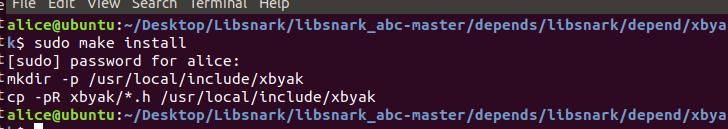
\includegraphics[width=1\linewidth]{image.png}
    \label{fig:placeholder}
\end{figure}
7）安装子模块 ate-pairing：
\begin{lstlisting}[language=bash]
# 在 depends/libsnark/depends/ate-pairing 目录下
make -j
test/bn
\end{lstlisting}
执行make -j最后几行结果如下：
\begin{figure}[H]
    \centering
    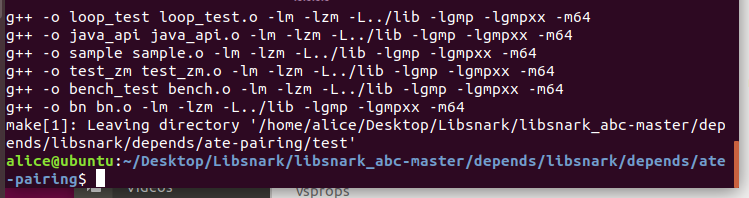
\includegraphics[width=1\linewidth]{image1.png}
    \label{fig:placeholder}
\end{figure}
执行test/bn最后几行结果如下：
\begin{figure}[H]
    \centering
    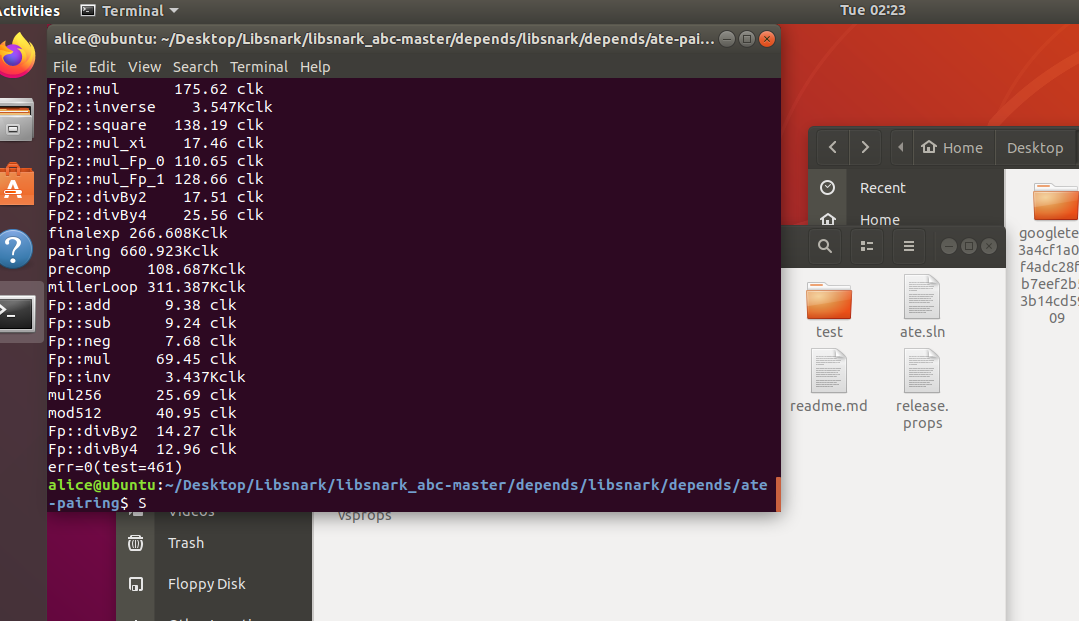
\includegraphics[width=1\linewidth]{image2.png}
    \label{fig:placeholder}
\end{figure}
8）安装子模块 libsnark-supercop：
\begin{lstlisting}[language=bash]
# 在 depends/libsnark/depends/libsnark-supercop 目录下
./do
\end{lstlisting}
出现以下代码，说明安装成功
\begin{figure}[H]
    \centering
    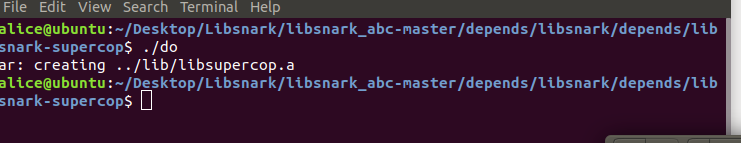
\includegraphics[width=1\linewidth]{image3.png}
    \label{fig:placeholder}
\end{figure}
9）安装子模块 gtest，将文件复制到 \texttt{depends/libsnark/depends/gtest}。

10）安装子模块 libff：
将下载得到的文件夹 Libff 内的文件复制到~/Libsnark/libsnark\_abcmaster/depends/libsnark/depends/libff。点击 libff->depends，可以看到一个 ate-pairing 文件夹
和一个 xbyak 文件夹，这是 libff 需要的依赖项。打开这两个文件夹，会发现它们是空的，
这时候需要将下载得到的 Ate-pairing 和 Xbyak 内的文件复制到这两个文件夹下。
在~/Libsnark/libsnark\_abc-master/depends/libsnark/depends/libff 下打开终端，执行命令:
\begin{lstlisting}[language=bash]
mkdir build && cd build
cmake ..
make
sudo make install
make check
\end{lstlisting}
如下图所示则安装成功：
\begin{figure}[H]    \centering
    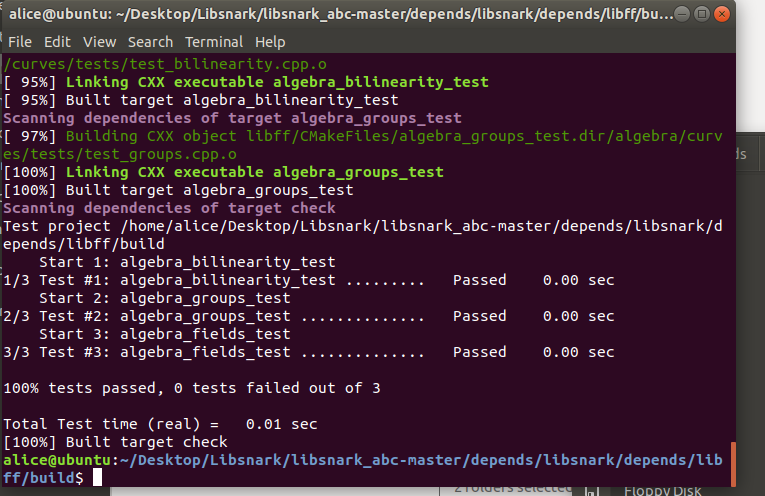
\includegraphics[width=1\linewidth]{image4.png}
    \label{fig:placeholder}
\end{figure}

11）安装子模块 libfqfft：
将下载得到的文件夹 Libfqfft 内的文件复制到~/Libsnark/libsnark\_abcmaster/depends/libsnark/depends/libfqfft。点击 libfqfft->depends，可以看到 libfqfft 有四个依
赖项，分别是 ate-pairing、gtest、libff、xbyak，点开来依然是空的。和上一步一样，将下
载得到的文件夹内文件复制到对应文件夹下。注意 libff 里还有 depends 文件夹，里面的
ate-pairing 和 xbyaky 也是空的，需要将下载得到的 airing 和 Xbyak 文件夹内的文件复制进
去。
\begin{lstlisting}[language=bash]
mkdir build && cd build
cmake ..
make
sudo make install
make check
\end{lstlisting}
如下图所示则安装成功：
\begin{figure}[H]
    \centering
    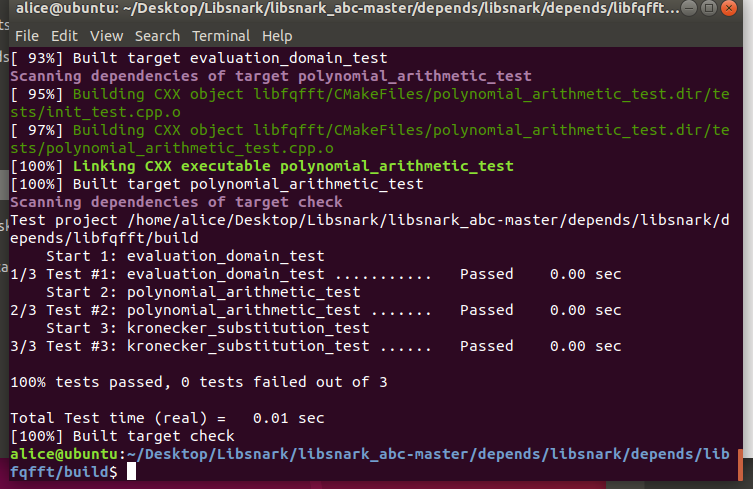
\includegraphics[width=1\linewidth]{image5.png}
    \label{fig:placeholder}
\end{figure}
12）libsnark 编译安装：
在~/Libsnark/libsnark\_abc-master/depends/libsnark 下打开终端，执行以下命令：
\begin{lstlisting}[language=bash]
# 在 depends/libsnark 目录下
mkdir build && cd build
cmake ..
make
make check
\end{lstlisting}
如下图所示则安装成功：
\begin{figure}[H]
    \centering
    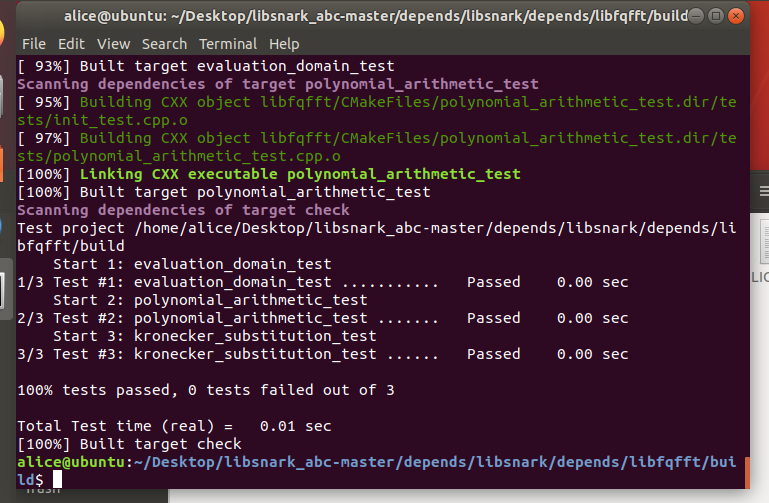
\includegraphics[width=1\linewidth]{image6.png}
    \label{fig:placeholder}
\end{figure}
13）整体编译安装：
\begin{lstlisting}[language=bash]
# 在 ~/Libsnark/libsnark_abc-master 目录下
mkdir build && cd build
cmake ..
make
\end{lstlisting}

14）运行环境测试：
\begin{lstlisting}[language=bash]
./src/test
\end{lstlisting}

最终出现如下日志，则说明已顺利拥有了 zkSNARK 应用开发环境，并成功跑了第
一个 zk-SNARKs 的 demo。
\begin{figure}[H]
    \centering
    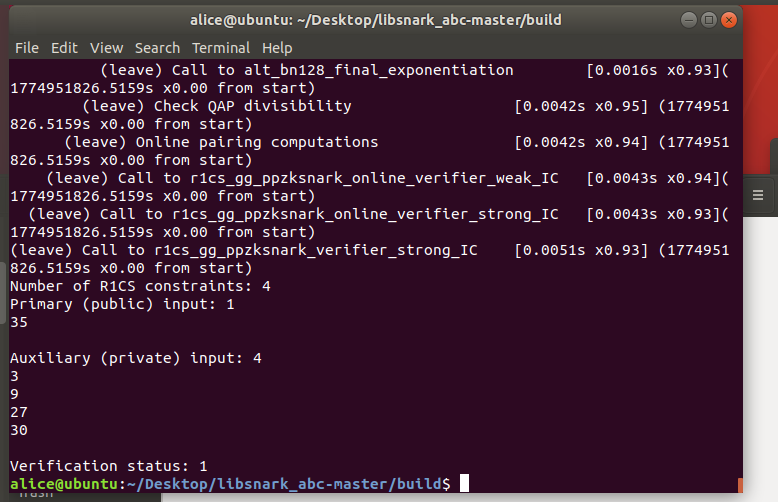
\includegraphics[width=1\linewidth]{image7.png}
\end{figure}
\subsection{算术电路设计与拍平}
针对待证明方程 $x^3 + x + 5 = 35$，将其拍平成多个 $x=y$ 或者 $x=y(op)z$ 形式的等式 ：
\begin{itemize}
    \item $w_1 = x \cdot x$
    \item $w_2 = w_1 \cdot x$
    \item $out = w_2 + x + 5$
\end{itemize}

\subsection{电路核心代码实现 (common.hpp)}
使用原型板 \texttt{protoboard} 搭建电路，代码放在公用文件 \texttt{common.hpp} 中 ：

\begin{lstlisting}[language=C++, caption={common.hpp 核心代码}]
#include <libsnark/common/default_types/r1cs_gg_ppzksnark_pp.hpp>
#include <libsnark/zk_proof_systems/ppzksnark/r1cs_gg_ppzksnark/r1cs_gg_ppzksnark.hpp>
#include <libsnark/gadgetlib1/pb_variable.hpp>
using namespace libsnark;
using namespace std;
typedef libff::Fr<default_r1cs_gg_ppzksnark_pp> FieldT;

protoboard<FieldT> build_protoboard(int* secret) {
    default_r1cs_gg_ppzksnark_pp::init_public_params();
    protoboard<FieldT> pb;
    pb_variable<FieldT> x, w_1, w_2, out;
    
    out.allocate(pb, "out");
    x.allocate(pb, "x");
    w_1.allocate(pb, "w_1");
    w_2.allocate(pb, "w_2");
    
    pb.set_input_sizes(1);
    pb.val(out) = 35;
    
    // 添加 R1CS 约束满足 a*b=c
    pb.add_r1cs_constraint(r1cs_constraint<FieldT>(x, x, w_1));         // x*x=w1
    pb.add_r1cs_constraint(r1cs_constraint<FieldT>(w_1, x, w_2));       // w1*x=w2
    pb.add_r1cs_constraint(r1cs_constraint<FieldT>(w_2 + x + 5, 1, out)); // (w2+x+5)*1=out
    
    if (secret != NULL) {
        pb.val(x) = secret[0];
        pb.val(w_1) = secret[0] * secret[0];
        pb.val(w_2) = secret[0] * secret[0] * secret[0];
    }
    return pb;
}
\end{lstlisting}

\subsection{密钥生成程序 (mysetup.cpp)}
此阶段生成证明密钥 \texttt{pk.raw} 和验证密钥 \texttt{vk.raw} ：

\begin{lstlisting}[language=C++, caption={mysetup.cpp}]
#include <fstream>
#include "common.hpp"
int main() {
    protoboard<FieldT> pb = build_protoboard(NULL);
    const r1cs_constraint_system<FieldT> cs = pb.get_constraint_system();
    const auto keypair = r1cs_gg_ppzksnark_generator<default_r1cs_gg_ppzksnark_pp>(cs);
    fstream pk("pk.raw", ios_base::out); pk << keypair.pk; pk.close();
    fstream vk("vk.raw", ios_base::out); vk << keypair.vk; vk.close();
    return 0;
}
\end{lstlisting}

\subsection{证明生成程序 (myprove.cpp)}
证明方 Alice 输入解 $x=3$ 构造证明文件 \texttt{proof.raw} ：

\begin{lstlisting}[language=C++, caption={myprove.cpp}]
#include <fstream>
#include "common.hpp"
int main() {
    int x; cout << "输入秘密值 x: "; cin >> x;
    int secret[3] = {x, x*x, x*x*x};
    protoboard<FieldT> pb = build_protoboard(secret);
    fstream f_pk("pk.raw", ios_base::in);
    r1cs_gg_ppzksnark_proving_key<libff::default_ec_pp> pk; f_pk >> pk; f_pk.close();
    const auto proof = r1cs_gg_ppzksnark_prover<default_r1cs_gg_ppzksnark_pp>(pk, pb.primary_input(), pb.auxiliary_input());
    fstream pr("proof.raw", ios_base::out); pr << proof; pr.close();
    return 0;
}
\end{lstlisting}

\subsection{验证程序 (myverify.cpp)}
验证方使用 \texttt{vk.raw} 与公有输入对证明进行校验 ：

\begin{lstlisting}[language=C++, caption={myverify.cpp}]
#include <fstream>
#include "common.hpp"
int main() {
    protoboard<FieldT> pb = build_protoboard(NULL);
    fstream f_vk("vk.raw", ios_base::in);
    r1cs_gg_ppzksnark_verification_key<libff::default_ec_pp> vk; f_vk >> vk; f_vk.close();
    fstream f_pr("proof.raw", ios_base::in);
    r1cs_gg_ppzksnark_proof<libff::default_ec_pp> proof; f_pr >> proof; f_pr.close();
    bool verified = r1cs_gg_ppzksnark_verifier_strong_IC<default_r1cs_gg_ppzksnark_pp>(vk, pb.primary_input(), proof);
    cout << "验证结果: " << verified << endl;
    return 0;
}
\end{lstlisting}

\subsection{编译运行与配置}
在 \texttt{src} 目录下创建上述文件。随后打开 \texttt{CMakeLists.txt}，在末尾追加如下代码 ：

\begin{lstlisting}[language=make, caption={CMakeLists.txt 追加配置}]
# mysetup
add_executable(mysetup mysetup.cpp)
target_link_libraries(mysetup snark)
target_include_directories(mysetup PUBLIC ${DEPENDS_DIR}/libsnark ${DEPENDS_DIR}/libsnark/depends/libfqfft)

# myprove
add_executable(myprove myprove.cpp)
target_link_libraries(myprove snark)
target_include_directories(myprove PUBLIC ${DEPENDS_DIR}/libsnark ${DEPENDS_DIR}/libsnark/depends/libfqfft)

# myverify
add_executable(myverify myverify.cpp)
target_link_libraries(myverify snark)
target_include_directories(myverify PUBLIC ${DEPENDS_DIR}/libsnark ${DEPENDS_DIR}/libsnark/depends/libfqfft)
\end{lstlisting}
\begin{figure}
    \centering
    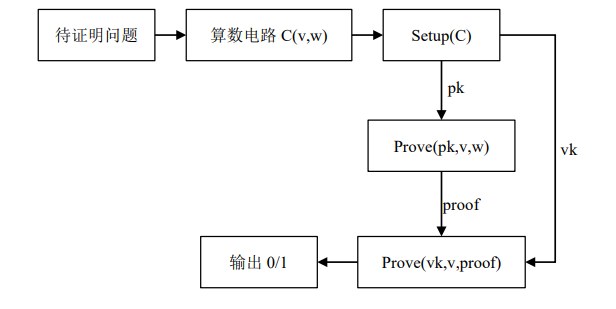
\includegraphics[width=1\linewidth]{image10.png}
\end{figure}
在 \texttt{build} 目录下执行编译并运行流程 ：
\begin{lstlisting}[language=bash]
cmake ..
make
cd src
./mysetup
./myprove
# 输入 3
./myverify
\end{lstlisting}
运行结果如下：验证结果为 1，表示证明方提供的私密输入 $x = 3$ 满足方程 $x^3 + x + 5 = 35$。该结果证实了证明方确实掌握该方程的有效解，且在不泄露 $x$ 具体数值的情况下，通过了零知识证明的验证 
\begin{figure}[H]
    \centering
    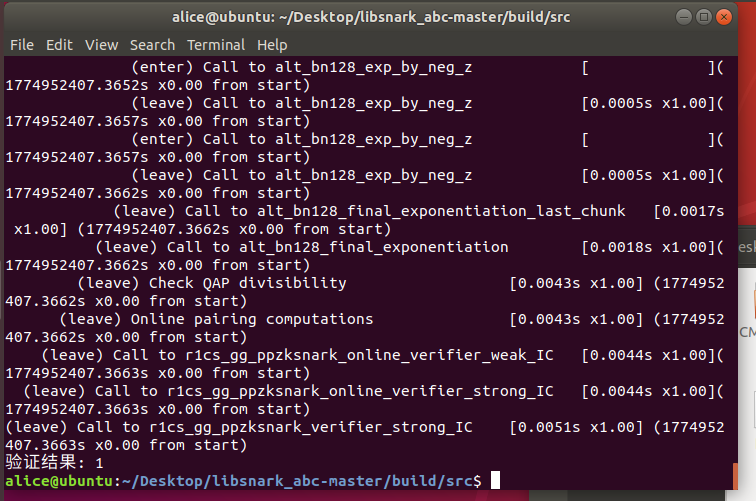
\includegraphics[width=1\linewidth]{image8.png}
\end{figure}

\section{总结}
通过复刻教材步骤，我完整实现了针对方程 $x^3+x+5=35$ 的零知识证明系统。实验加深了对电路拍平、R1CS 约束构建以及 zkSNARK 三阶段流程的理解 。虽然环境配置过程复杂，但最终通过 Setup-Prove-Verify 全流程，成功验证了证明方的解，充分体现了零知识证明在数据安全领域的应用价值。

% --- 正文结束 ---





\end{document}